% V5.0 do not change this line
\section{Proposed Measurements} 
%

We propose to use the same experimental setup of E12-09-019 experiment. 
We will add a kinematic point at \qsq~= 4.5 \gevcsq, but with a higher $\epsilon$ value. 
This additional point along with the data point of E12-09-019 experiment will allow us to perform LT separation and 
obtain (in one-photon approximation) the \gen~value. 
Table.~VIII %\ref{tab:table1}
displays the kinematic setting of the proposed experiment. 
%
\begin{center}
\begin{table}[h]
\begin{tabular}{|c|c|c|c|c|c|c|c|c|}
\hline
\small{Point} & $Q\textsuperscript{2}$  & E & E$'$  & $\theta_{BB}$ & $\theta_{SBS}$ & $\epsilon$ &$\Delta \sigma$ & $\Delta TPE$\\
& (GeV/c)$^2$ & (GeV) & (GeV)  & degrees & degrees   &  & (\%)& (\%) \\
\hline
\textcolor{blue}
 1&\textcolor{blue} {4.5} & \textcolor{blue}{4.4} & \textcolor{blue}{2.0} & \textcolor{blue}{41.88}  & \textcolor{blue}{24.67} & \textcolor{blue}{0.599} & & \\
\hline
2 & 4.5  &  6.6  &  4.2  & 23.23  &  31.2  &  0.838 & & \\
\hline
\end{tabular} 
\caption{Kinematic settings of the proposed experiment. The blue row is a kinematic point of E12-09-019 experiment.}
\label{tab:table1}
\end{table}
\end{center}
%
\begin{figure}[!h]
  \begin{center}
    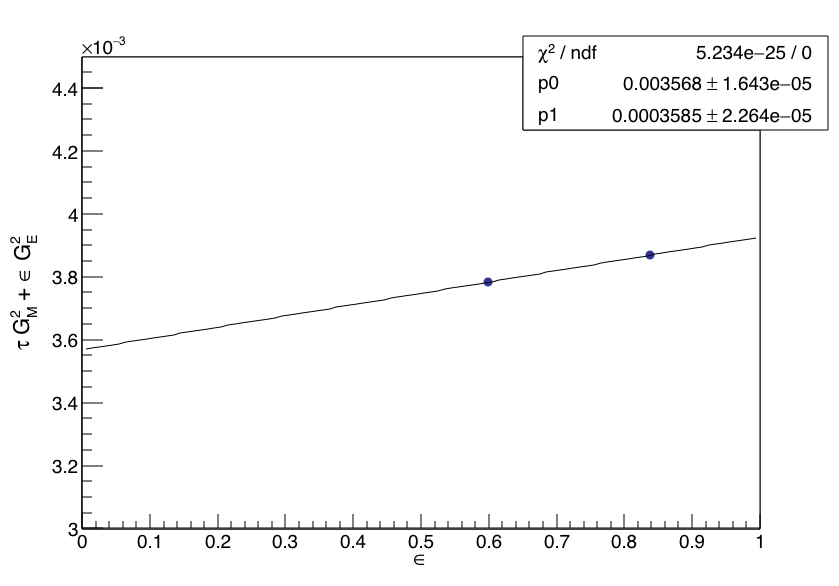
\includegraphics[width=7cm]{Plots/reduced.png}
    \caption{The reduced cross section (model) as a function of $\epsilon$}
    \label{fig:sigmaR_feps}
  \end{center}
\end{figure}
%
%
The reduced cross section
%
\begin{equation}
  \sigma_R = %F^2 \times \epsilon(1+\tau) =
  \epsilon G_E^2 + \tau G_E^2 
\end{equation}
%
is displayed as a function of $\epsilon$ on Fig.~12.%\ref{fig:sigmaR_feps}.
Admitting the prediction from~\cite{Blunden:2005ew}, the neutron two-photon exchange contribution would amount to $0.069 \pm 0.010(stat.) \pm 0.012(syst.)$, which would be a $\geq~4~\sigma$ observation of this quantity.
